\documentclass{ximera}  


\input{../preamble.tex}



 
\title{Grounding and Shielding} 
\author{Milica Markovic} 
\outcome{Students will }
\begin{document}  
\begin{abstract}  

\end{abstract}  
\maketitle    


\section{Grounding}



   \begin{question}
 The four equations below show the tangential and normal electric field at the boundary of two dielectrics. Dielectric 1 is a Teflon with a relative dielectric constant of 2.2, and dielectric 2 is Silicon with a relative dielectric constant of 11.2. Which set of equations represents a possible electric field? 
   \begin{multipleChoice}
     \choice{$2.2 \,E_{1t}= 11.2 \,E_{2t}$ and $E_{1n}=  E_{2n}$}
     \choice[correct]{$E_{1t}=E_{2t}$ and $2.2 \,E_{1n}= 11.2 \,E_{2n}$ }
     \choice{$2.2 \,E_{1t}= 11.2 \,E_{2t}$ and $ E_{1n}= E_{2n}$}
     \choice{$E_{1t}=E_{2t}$ and $11.2 \, E_{1n}= 2.2 \, E_{2n}$}
   \end{multipleChoice}
   \end{question}
   






\begin{figure}[htbp]
\begin{center}
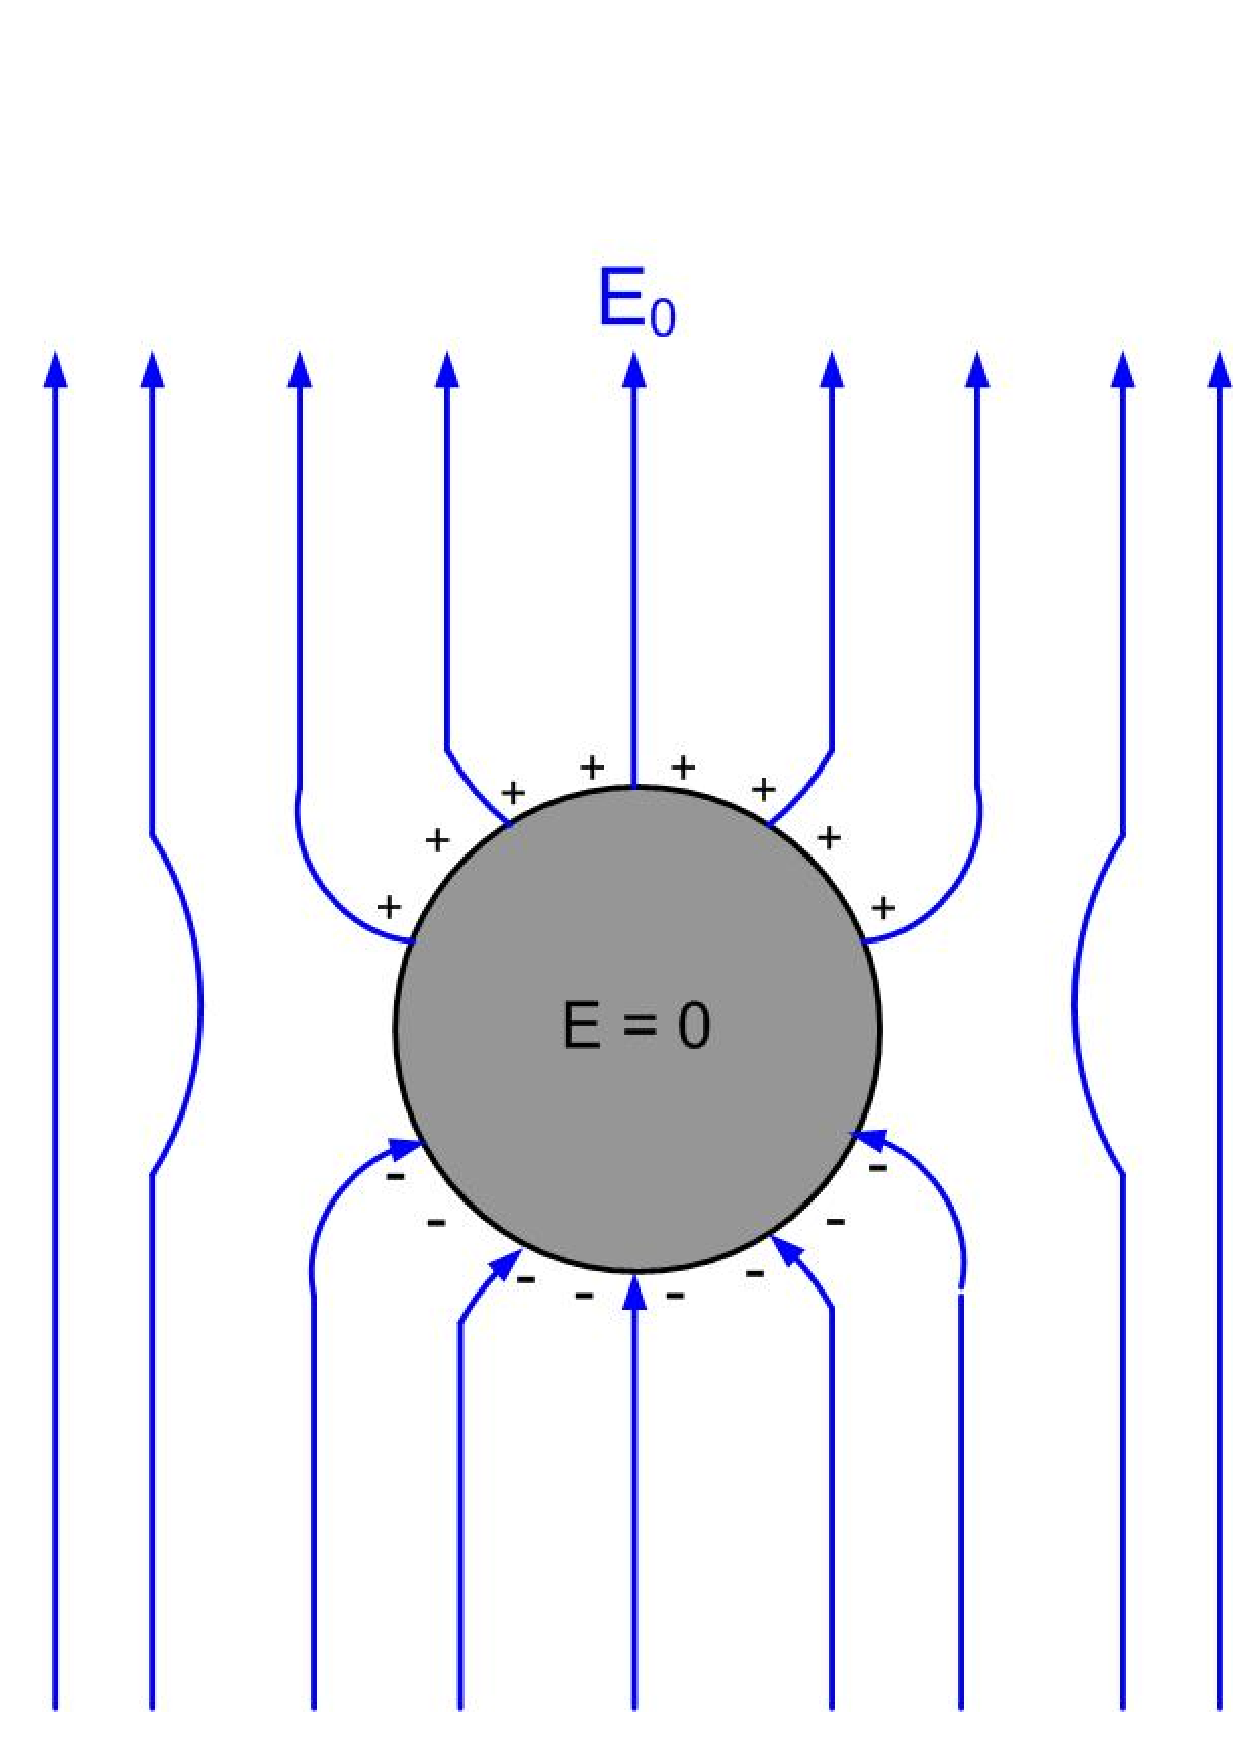
\includegraphics[scale=0.5]{../jpg/metalsphereinefield.jpg}
\end{center}
\caption{Metallic sphere in an external electric field.}
\label{fig:Grounding}
\end{figure}



\section{Shielding}







\end{document} 

